\documentclass[conference]{IEEEtran}
\IEEEoverridecommandlockouts
% The preceding line is only needed to identify funding in the first footnote. If that is unneeded, please comment it out.
\usepackage{cite}
\usepackage{amsmath,amssymb,amsfonts}
\usepackage{algorithmic}
\usepackage{graphicx}
\usepackage{dblfloatfix}
\usepackage{subcaption}

%\def\BibTeX{{\rm B\kern-.05em{\sc i\kern-.025em b}\kern-.08em
%    T\kern-.1667em\lower.7ex\hbox{E}\kern-.125emX}}
\begin{document}

\title{Robust Many-to-Many Location Sharing Based on Diffie-Hellman Encrypted Key Exchange \\
%{\footnotesize \textsuperscript{*}Note: Sub-titles are not captured in Xplore and
%should not be used}
%\thanks{Identify applicable funding agency here. If none, delete this.}
}

%\author{\IEEEauthorblockN{Shuai Fu}
%\IEEEauthorblockA{\textit{Faculty of Engineering and Computer Science}\\
%\textit{Concordia University}\\
%Montreal, Canada\\
%f\_shuai@encs.concordia.ca}
%\and
%\IEEEauthorblockN{Nizar Bouguila}
%\IEEEauthorblockA{\textit{Concordia Institute for Information Systems Engineering} \\
%\textit{Concordia University}\\
%Montreal, Canada \\
%bouguila@ciise.concordia.ca}
%}

\maketitle

\begin{abstract}
A novel unsupervised Bayesian image categorization framework based on asymmetric Gaussian mixture (AGM) model is proposed and the mixture parameter estimation is achieved by sampling-based reversible jump Markov chain Monte Carlo (RJMCMC) method. Previous researches have reveled that AGM outperforms classic symmetric mixture models (i.e Gaussian mixture model (GMM)) since the model adapts both symmetric and asymmetric datasets yielding better fitting accuracy. Moreover, the introduction of RJMCMC, a hybrid self-adapted sampling-based MCMC implementation, enables model transfer throughout parameter learning process, therefore, automatically converges to the optimal number of categories. In order to better identify visual features from the challenging UIUC sport events dataset, the image representative data is generated by adopting scale-invariant feature transform (SIFT), bag-of-visual-words (BOVW) and probabilistic latent semantic analysis (pLSA) techniques. Eventually, irrelevant and unneeded information will be filtered by feature selection. A comparison between AGM and other popular classifiers is given to discover its merits and the direction of future work is suggested.
\end{abstract}

\begin{IEEEkeywords}
Asymmetric Gaussian Mixture, Image Categorization, RJMCMC, SIFT, BOVW, pLSA 
\end{IEEEkeywords}

\section{Introduction}
Recently, as the consequence of frequent usage of mobile phone, social media and cloud storage, digitalized visual data such as photos and pictures brings difficulties for management and analysis. Unlike those within text-based documents, indexing and comparison among images could be challenging. Therefore, image categorization is becoming one of the most interesting research topics in computer vision community. Indeed, finding relevant images from a rapidly growing unannotated image database is challenging which makes the previous time-consuming manual categorization methods infeasible. Automated methods such as machine-learning-based approaches \cite{Han2005} introduce image representation methodologies for visual feature extraction and both generative and discriminative classifiers for categorization. Meanwhile, modern machine-learning-based solutions can be divided into two main streams, classification-based supervised and clustering-based unsupervised ones. Compared to supervised solutions, unsupervised approach has no assumption on the number of groups, therefore, friendly to new added images and categories which makes it more suitable for increasing datasets. Moreover, it also immunizes against learning biases and overfitting problems that commonly exist in most supervised approaches if model training is inappropriate. Consequently, unsupervised categorization of images or image parts \cite{Fan2011a,Bouguila2011,Azam2015} acts an important role for image and video summarization, human action recognition, and image search etc,. It can also be seen as a pre-processing step for supervised methodologies for classification or segmentation. As upgrade of single-mathematical-model-based methodologies, mixture models \cite{Yang2015,Wen2015,Bouguila2011a} can be seen as a superimposition of certain mixture components sharing dependencies with each other, therefore, lead to outstanding performance especially for high-dimensional and multi-cluster datasets. More precisely, for Gaussian-like datasets, Gaussian mixture model (GMM)\cite{Richardson1997} demonstrated satisfactory fitting abilities on applications such as computer vision, pattern recognition and data mining. However, under a more general circumstances regarding to non-Gaussian or asymmetric datasets, asymmetric Gaussian mixture (AGM) model \cite{Elguebaly2014} leads to a better accuracy by introducing two variance parameters for both left and right parts of asymmetric Gaussian distribution, providing more flexibility for variant real applications. Therefore, the justification of choosing AGM model and its merits will be discussed in the following chapters.

As an essential step for mixture model in practise, parameter estimation could be challenging and highly affects the performance. One of the most popular learning algorithm is the maximum-likelihood-based expectation maximization (EM) \cite{Dempster1977} which has been proven as effective under some circumstances. However, as a deterministic solution, the efficiency and usability of EM could be significantly compromised by bad initialization and overfitting problems \cite{Bouguila2009} \cite{Bouguila2012} which usually cause slow convergence and improper approximation, and eventually, compromise the accuracy of the model. As a consequence, researchers are paying more attention to sampling-based stochastic Bayesian learning algorithms \cite{Bourouis2014,Bouguila2008}, such as Markov Chain Monte Carlo (MCMC) based implementations\cite{Fu2018a} to address previous issue by introducing prior and posterior distributions for every mixture parameter which decouple the dependencies between mixture parameters and mixture components, therefore, allow model adjustment by substituting proposed distributions to adapt to varied application datasets in a more flexible way \cite{Bouguila2007,Fu2018}. Accordingly, we chose an advanced MCMC implementation called reversible jump MCMC (RJMCMC)\cite{Bouguila2012} which is based on a hybrid Metropolis-Hastings within Gibbs sampling\cite{Bouguila2009} solution, combining both Metropolis-Hastings \cite{Hastings1970} and Gibbs sampling \cite{Geman1987} methods because the main difficulty of applying traditional MCMC method is that, under some circumstances, direct sampling is not always straightforward that distributions of mixture parameters are latent and dependencies between parameters are unknown. By integrating the merits of both methods, mixture parameters will be evaluated iteratively and, eventually, the optimal parameter values will be identified after convergence. Furthermore the self-adapted learning process \cite{Bouguila2012} treats component number as an extra parameter and adjust it throughout iterations by automatically increasing (component birth/death step) and decreasing (component merge/split step) according to current status, therefore, enables model transfer which significantly improves the learning performance. 

Before deploying UIUC sports event database \cite{Li2007} to validate AGM framework, image processing is needed because images should be represented as visual features and, eventually, be translated into numerical data. For this reason, we decided to adopt scale-invariant feature transform (SIFT) \cite{Lowe1999} to detect and describe image features even under changes in image scale, noise and illumination. However, generated SIFT features have to be categorized and features belong to each image should be counted as histograms to be the input of AGM model. Therefore, bag-of-visual-words \cite{Fei-Fei2005} and probabilistic latent semantic analysis (pLSA)\cite{Hofmann2001} are responsible for the generation of feature histogram and reduction of dimensionality.

The next sections are organized as follows. Section II and III elaborate the AGM model and its Bayesian learning algorithm. Section IV is devoted to results analysis and Section V gives a conclusion of the paper and proposes future research directions. 


\section{Asymmetric Gaussian Mixture Model}
The likelihood function of AGM model\cite{Elguebaly2014} with $M$ mixture components can be illustrated as follows:

\begin{align}
p(\mathcal{X}|\Theta) = \prod_{i=1}^N \sum_{j=1}^Mp_jp(X_i|\xi_j)
\label{eq:likelihood}
\end{align}

where $\mathcal{X} = (X_1,...,X_N)$ reprensents the dataset with $N$ observations, $\Theta = \{p_1,...,p_M, \xi_1,...,\xi_M\}$ defines the mixture parameters set of AGM mixture model including component weight $p_j$ (0 $< p_j \leq$ 1 and $\sum_{j=1}^Mp_j$ = 1) and asymmetric Gaussian distribution (AGD) parameters set $\xi_j$ for mixture component $j$. Assuming the dataset $\mathcal{X}$ is $d$-dimensional, for each observation $X_n = (x_{n1},...,x_{nd})\in\mathcal{X}$, the probability density function\cite{Elguebaly2014} for $j$-th component of the model can be defined as follows:

\begin{multline}
p(X_n|\xi_j) \propto \prod_{k=1}^{d} \frac{1}{(\sigma_{l_{jk}}+\sigma_{r_{jk}})} \\
\times \left\{\begin{matrix}
\exp \begin{bmatrix}
-\frac{(x_{nk}-\mu_{jk})^2}{2(\sigma_{l_{jk}})^2}
\end{bmatrix}\ if\ x_{nk}\ <\ \mu_{jk} \\ 
\exp \begin{bmatrix}
-\frac{(x_{nk}-\mu_{jk})^2}{2(\sigma_{r_{jk}})^2}
\end{bmatrix}\ if\ x_{nk}\ \geqslant\ \mu_{jk} \\ 
\end{matrix}\right.
\label{eq:pdf}
\end{multline}

parameters set of component $j$ is $\xi_j = (\mu_j,\sigma_{lj},\sigma_{rj})$ where $\mu_j = (\mu_{j1},...,\mu_{jd})$ is the mean, $\sigma_{lj} = (\sigma_{lj1},...,\sigma_{ljd})$ and $\sigma_{rj} = (\sigma_{rj1},...,\sigma_{rjd})$ represents the left and right standard deviation vectors of AGD . 

We bring a $M$-dimensional membership vector $Z$ to each observation $X_i\in\mathcal{X}, Z_i = (Z_{i1},...,Z_{iM})$, indicating which specific component $X_i$ belongs to\cite{Bouguila2006}, such that:
\begin{align}
Z_{ij} = \left\{\begin{matrix}
1\qquad\mbox{ if }X_i\mbox{  belongs to component }j \\
0\qquad\quad\qquad \mbox{otherwise} \qquad\qquad\quad\quad \\
\end{matrix}\right.
\label{eq:memVector}
\end{align}
that being said, $Z_{ij} = 1$ only when observation $X_i$ has the highest probability of belonging to component $j$ and accordingly, for other components, $Z_{ij} = 0$. 

Hence, the complete likelihood function can be obtained by combining Eq. \eqref{eq:likelihood} and Eq. \eqref{eq:memVector} as follows:
\begin{align}
p(\mathcal{X}, Z|\Theta) = \prod_{i=1}^{N}\prod_{j=1}^{M}(p_jp(X_i|\xi_j))^{Z_{ij}}
\label{eq:compPdf}
\end{align}


\subsection{Priors and Posteriors}
As mentioned before, MH-within-Gibbs based RJMCMC learning algorithm implementation introduces definitions of priors and posteriors for mixture weights and parameters to avoid direct sampling. For a specific iteration $t$, since mixture weight $p_j$ satisfies 0 $< p_j \leq$ 1 and $\sum_{j=1}^Mp_j$ = 1, a natural choice of the prior is Dirichlet distribution\cite{Elguebaly2013} as follows:
\begin{align}
\pi(p_j^{(t)}) \sim \mathcal{D}(\gamma_1,...,\gamma_M )
\label{eq:priorWeight}
\end{align}

where $\gamma = \gamma_j = \dots = \gamma_M$ is a known hyperparameter. By taking the membership vector Z into account as a condition, the posterior probability of mixture weight $p_j$ is defined as follows:
\begin{align}
p(p_j^{(t)}|Z^{(t)}) \sim \mathcal{D}(\gamma_1 + n_1^{(t)},...,\gamma_M + n_M^{(t)})
\label{eq:posterWeight}
\end{align}

where $n_j$ represents the number of observations of component $j$ which could be calculated using membership vectors as follows:
\begin{align}
n_j^{(t)} = \sum_{i=1}^NZ_{ij}\ (j = 1,...,M) 
\label{eq:nj}
\end{align}

The sampling process of mixture parameters employs the same concept. The proposal posterior distribution is  $\xi^{(t)} \sim q(\xi|\xi^{(t-1)})$. More specifically, for parameters of AGM model $\xi^{(t)} = (\mu^{(t)}, \sigma_{l}^{(t)}, \sigma_{r}^{(t)})$, we choose $d$-dimensional Gaussian distributions as posterior distributions respectively:
\begin{multline}
\qquad\qquad\qquad\qquad\mu_j^{(t)} \sim \mathcal{N}_d(\mu_j^{(t-1)},\Sigma) \\
\qquad\sigma_{lj}^{(t)} \sim \mathcal{N}_d(\sigma_{lj}^{(t-1)},\Sigma) \\
\sigma_{rj}^{(t)} \sim \mathcal{N}_d(\sigma_{rj}^{(t-1)},\Sigma)\qquad\qquad\quad
\label{eq:posters}
\end{multline}

where $\Sigma$ is $d$ x $d$ identity matrix which makes the sampling a random walk MCMC process. Correspondingly, the priors are $\mu \sim \mathcal{N}_d(\eta,\Sigma)$ and $\sigma_l, \sigma_r \sim \mathcal{N}_d(\tau,\Sigma)$ given known hyperparameters $\eta$ and $\tau$.

\subsection{Feature Selection}
The AGM model defined in Eq. \eqref{eq:likelihood} assumes that all the $d$ features of observations have the same weight of importance and carry pertinent information which is not always the case and many of those features can be irrelevant for clustering purpose. In order to tackle this problem and define relevance and importance of features, feature selection techniques \cite{Elguebaly2013}\cite{Elguebaly2015a} should be taken into consideration. By denoting background Gaussian distributions for all the $d$ features with parameter set $\Psi = \{\mu'_1,...,\mu'_d, \sigma'_1,...,\sigma'_d\}$, where $\mu'$ and $\sigma'$ represent the mean and standard deviation of the Gaussian distribution respectively. Then, Eq. \eqref{eq:likelihood} can be reformulated with the feature relevancy approach suggested in Ref. \cite{Law2004} as follows:

\begin{align}
p(\mathcal{X}|\Theta,\Psi,\Phi) = \prod_{i=1}^N \sum_{j=1}^Mp_j\prod_{k=1}^dp(X_{ik}|\xi_{jk})^{\phi_k}p(X_{ik}|\psi_{k})^{1-\phi_k}
\label{eq:likelihoodFeature}
\end{align}

where $\psi_k=(\mu'_k,\sigma'_k)$ and $\Phi = (\phi_1,\dots,\phi_d)$ is a binary relevancy vector where $\phi_k=1$ if $k$-th feature is relevant or $\phi_k=0$ otherwise. If we consider the relevancy vector $\Phi$ as a latent variable, the complete likelihood function of AGM model with full parameter set will be given as follows:

\begin{align}
p(\mathcal{X}|\Theta') = \prod_{i=1}^N \sum_{j=1}^Mp_j\prod_{k=1}^d[\omega_kp(X_{ik}|\xi_{jk})+(1-\omega_k)p(X_{ik}|\psi_{k})]
\label{eq:likelihoodFeatureComp}
\end{align}

where $\Theta'=(\Theta,\Psi,\Omega)$ and $\Omega = (\omega_1,\dots,\omega_d)$ is the relevancy weight with value range of $0 \leq \omega_d \leq 1$ which represents the probability that $k$-th feature is relevant. Finally, the calculation of relevancy weight $\omega_k$ is given as follows:

\begin{align}
\omega_k = \frac{\sum_{j=1}^Mp_jp(X_{k}|\xi_{jk})}{\sum_{j=1}^Mp_jp(X_{k}|\xi_{jk})+\sum_{j=1}^Mp_jp(X_{k}|\psi_{k})}
\label{eq:releWeight}
\end{align}

Therefore, irrelevant features only have few contribution for the clustering process, thus the usability of AGM model is extended to more common and complicated cases such as high-dimensional noisy applications.

\section{Bayesian Learning Algorithm via RJMCMC}
\subsubsection*{MH-within-Gibbs}
MH-within-Gibbs method, a sampling-based learning algorithm,  performs random sampling from posteriors of parameters, and then calculates the acceptance ratio $r$ in order to make a decision whether the new samples should be accepted or discarded for next iteration. Due to the usage of membership vector $Z$, the mixture weight $p_j$ can be derived within Gibbs sampling part. Therefore, it will be excluded from the calculation of the acceptance ratio $r$ which is defined as follows:
\begin{align}
r = \frac{p(\mathcal{X}|\Theta^{(t)})\pi(\Theta^{(t)})q(\Theta^{(t-1)}|\Theta^{(t)})}{p(\mathcal{X}|\Theta^{(t-1)})\pi(\Theta^{(t-1)})q(\Theta^{(t)}|\Theta^{(t-1)})}
\label{eq:r}
\end{align}

Further information about the calculation of acceptance ratio
$r$ is explained in Appendix A. Once acceptance ratio $r$ is derived, acceptance probability $\alpha = min[1,r]$ \cite{Luengo2013} could be computed. Then $u \sim U_{[0,1]}$ is supposed to be generated randomly. If $\alpha < u$, the proposed move should be accepted and parameters should be updated by $p^{(t)}$ and $\xi^{(t)}$ for next iteration. Otherwise, we discard $p^{(t)}$, $\xi^{(t)}$ and set $p^{(t)} = p^{(t-1)}$, $\xi^{(t)} = \xi^{(t-1)}$. 
\bigskip

\begin{figure}[b]
\centering
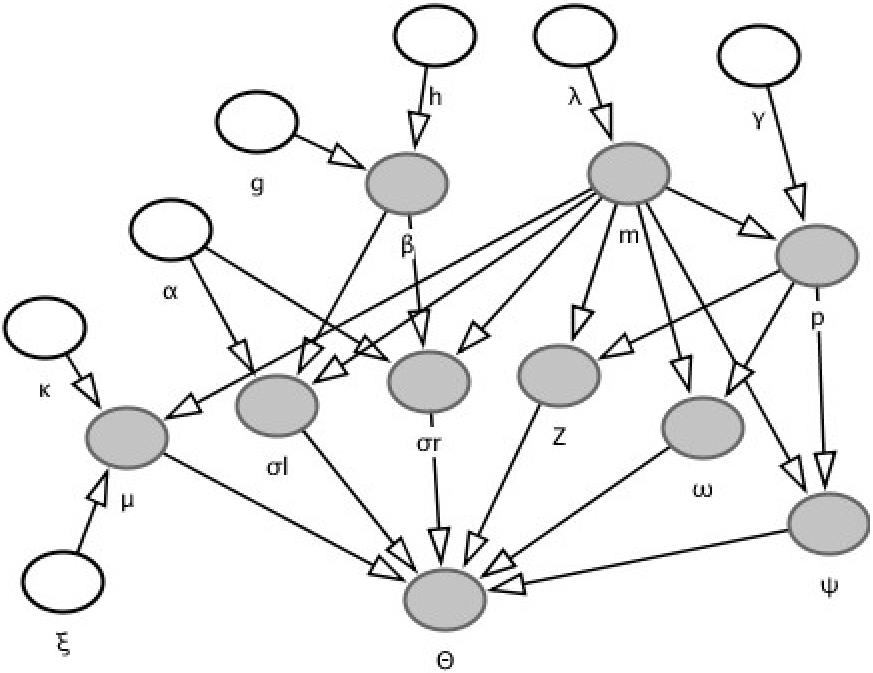
\includegraphics[width=0.4\paperwidth]{DAG_feature.jpg}
\caption{DAG of RJMCMC Bayesian parameter learning network}
\label{fig:1}
\end{figure}

\begin{figure}[b]
    \centering
    \begin{subfigure}[b]{0.2\paperwidth}
        \centering
        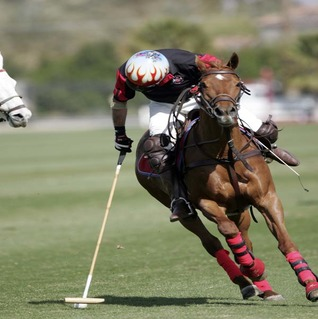
\includegraphics[width=0.15\paperwidth]{polo.jpg}
        \caption{}
    \end{subfigure}
    \begin{subfigure}[b]{0.2\textwidth}
        \centering
        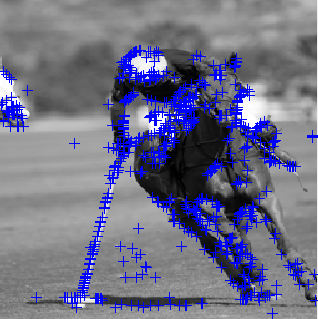
\includegraphics[width=0.15\paperwidth]{polo_sift.png}
        \caption{}
    \end{subfigure}
    \caption{a) Original UIUC sport image. b) Enhanced image with SIFT extracted visual features.}\label{fig:2}
\end{figure}



\subsubsection*{RJMCMC moves}
Traditional MH-within-Gibbs algorithm assumes that the component number $M$ is given and persistent throughout the learning process. However, because of bad initialization or just information leakage, $M$ could be inaccurate or unknown. Under these circumstances, RJMCMC algorithm presents its merits by providing extra four independent steps (birth/death steps and merge/split steps) into learning process which could change component number $M$, therefore, brings more generalities. 

In practice, within every RJMCMC learning iteration, the current component number $m$ is considered as an extra parameter which has a proposed Poisson prior $\mathcal{P}(\lambda)$ with $\lambda = 4$ particularly in our case \cite{Richardson1997}. Accordingly, let $M_{min}$ and $M_{max}$ denote the minimum and maximum number of components $M$, and assume the probabilities of performing birth/split and death/merge steps are $b_m$ and $d_m = 1 - b_m$ for $m = M_{min},\dots,M_{max}$ respectively. Obviously, $b_{M_{max}}=0$ and $d_{M_{min}}=0$. Correspondingly, $d_{M_{max}}=1-b_{M_{max}} = 1$ and $b_{M_{min}}=1-d_{M_{min}}=1$. For $m=M_{min}+1,\dots,M_{max}-1$, for simplification purpose, we choose the same value for both $b_m$ and $d_m$ as $b_m=d_m=0.5$. Within every iteration, we generate a random value $u' \sim U_{[0,1]}$ respectively for the four RJMCMC steps. If $b_m >= u'$ or $d_m >= u'$, birth/split or death/merge steps should be performed correspondingly \cite{Richardson1997}.

\textbf{Merge and Split Steps}: Randomly choose two components $(j_1,j_2)$ satisfying that $\mu_{j_1}<\mu_{j_2}$ with no other $\mu_j$ in the interval $[\mu_{j_1},\mu_{j_2}]$. The newly merged component $j'$ will contain the observations that previously belonged to both component $j_1$ and $j_2$. Meanwhile, reduce current value of component number $m$ to $m-1$, then calculate mixture weight and parameters for $j'$ as follows:
\begin{multline}
\qquad\qquad\qquad\qquad p_{j'} = p_{j_1}+p_{j_2} \\
p_{j'}\mu_{j'} = p_{j_1}\mu_{j_1} + p_{j_2}\mu_{j_2} \\
p_{j'}(\mu_{j'}^2 + \sigma_{j'l}^2) = p_{j_1}(\mu_{j_1}^2 + \sigma_{j_1l}^2)\qquad \\
\qquad\qquad+ p_{j_1}(\mu_{j_1}^2 + \sigma_{j_1l}^2) \\
p_{j'}(\mu_{j'}^2 + \sigma_{j'r}^2) = p_{j_1}(\mu_{j_1}^2 + \sigma_{j_1r}^2)\qquad\\
+p_{j_1}(\mu_{j_1}^2 + \sigma_{j_1r}^2)\qquad\qquad
\label{eq:merge}
\end{multline}

As a reverse of merge step, we split component $j'$ into two ($j_1$ and $j_2$) with 3 degrees of freedom $(u_1 \sim Beta(2,2), u_2 \sim Beta(2,2), u_3 \sim Beta(1,1))$ and, accordingly, increase $m$ to $m+1$. Therefore, mixture parameters for split components can be calculated as follows:
\begin{multline}
\qquad\qquad\qquad p_{j_1} = p_{j'}u_1, p_{j_2} = p_{j'}u_2 \\
\mu_{j_1} = \mu_{j'} - \frac{u_2(\sigma_{j'l}+\sigma_{j'r})}{2} \sqrt{\frac{p_{j_2}}{p_{j_1}}} \\
\mu_{j_2} = \mu_{j'} + \frac{u_2(\sigma_{j'l}+\sigma_{j'r})}{2} \sqrt{\frac{p_{j_1}}{p_{j_2}}} \\
\sigma_{j_1l}^2 = u_3(1-u_2^2)\sigma_{j'l}^2\frac{p_{j'}}{p_{j_1}} \\
\sigma_{j_1r}^2 = u_3(1-u_2^2)\sigma_{j'r}^2\frac{p_{j'}}{p_{j_1}} \\
\sigma_{j_2l}^2 = (1-u_3)(1-u_2^2)\sigma_{j'l}^2\frac{p_{j'}}{p_{j_2}} \\
\sigma_{j_2r}^2 = (1-u_3)(1-u_2^2)\sigma_{j'r}^2\frac{p_{j'}}{p_{j_2}} \qquad\quad
\label{eq:split}
\end{multline}

In order to decide whether the merge and split steps should be accepted or not, the acceptance probability \cite{Richardson1997} can be derived as follows: 

\begin{multline}
\mathcal{A}=\frac{p(\mathcal{X},Z|\Theta')}{p(\mathcal{X},Z|\Theta)}\frac{m'\mathcal{P}(m'|\lambda)}{\mathcal{P}(m|\lambda)}\frac{p_{j_1}^{\gamma-1+n_1}p_{j_2}^{\gamma-1+n_2}}{p_{j'}^{\gamma-1+n_1+n_2}Beta(\gamma,m\gamma)} \\
\times \sqrt{\frac{\kappa}{2\pi}} \exp[-\frac{1}{2}\kappa{(\mu_{j_1}-\xi)+(\mu_{j_2}-\xi)+(\mu_{j'}-\xi)}] \\
\times \frac{\beta^{\alpha}}{\Gamma(\alpha)}(\frac{\sigma_{j_1l}^2\sigma_{j_1r}^2\sigma_{j_2l}^2\sigma_{j_2r}^2}{\sigma_{j'l}^2\sigma_{j'r}^2})^{-\alpha-1} \qquad\qquad\qquad\qquad\\
\times \exp [{-\beta(\sigma_{j_1l}^2+\sigma_{j_1r}^2+\sigma_{j_2l}^2+\sigma_{j_2r}^2-\sigma_{j'l}^2-\sigma_{j'r}^2)}] \\
\qquad\times \frac{d_{m'}}{b_mP_{alloc}} [Beta(\mu_1|2,2)Beta(\mu_2|2,2)Beta(\mu_3|1,1)]^{-1} \\
\times \frac{p_{j'}|\mu_{j_1}-\mu_{j_2}|\sigma_{j_1l}^2\sigma_{j_1r}^2\sigma_{j_2l}^2\sigma_{j_2r}^2}{\mu_2(1-\mu_2^2)\mu_3(1-\mu_3)\sigma_{j'l}^2\sigma_{j'r}^2} \qquad\qquad\qquad\quad
\label{eq:acptProMS}
\end{multline}
where $\Theta'$ and $m' = m + 1$ denote the mixture parameters set and the component number respectively before merge or after split steps. $\kappa$ is a known hyperparameter and $\xi$ is the midpoint of the variation interval of the involved data observations. Besides, $P_{alloc}$ is the probability of which this particular allocation is made. Therefore, the acceptance probability for merge step is $\min(1,\mathcal{A})$ and, correspondingly, for split step is $\min(1,\mathcal{A}^{-1})$.

\textbf{Birth and Death Steps}: Compared to merge and split steps, birth and death steps are relatively straightforward because the newborn and dead components are empty ones which means parameter re-calculation is not needed. Mixture weight $p_{new}$ in birth step can be obtained by sampling from Beat distribution $p_{new} \sim Beta(1,m)$ and mixture parameters can be derived from the priors as follows\cite{Casella2004}:
\begin{align}
\mu \sim \mathcal{N}(\xi,\kappa^{-1}), \quad \sigma_{l}^{-2},\sigma_{r}^{-2} \sim \Gamma(\alpha,\beta), \quad \beta \sim \Gamma(g,h)
\label{eq:prior}
\end{align}
where hyperparameters $\kappa$, $\alpha$, $g$ and $h$ are estimated by data. For death step, an empty component should be randomly selected and deleted among the existing components if there is any. Otherwise, this step will be skipped. After birth and death steps, mixture weights $p_j$ should be re-scaled so that all weights sum to 1. Acceptance probability for birth and death steps is also required as the one for merge and split steps whose definition is as follows:

\begin{multline}
\mathcal{A}'=\frac{\mathcal{P}(m'|\lambda)}{\mathcal{P}(m|\lambda)}\frac{1}{Beta(m\gamma,\gamma)}p_{j'}^{\gamma-1}(1-p_{j'})^{N+m\gamma-m}m' \\
\times \frac{d_{m'}}{(m_0+1)b_m}\frac{1}{Beta(p_{j'}|1,m)}(1-p_{j'})^m\qquad\quad
\label{eq:acptProBD}
\end{multline}
where $m_0$ is the amount of empty components. Thus, the probabilities of occurrence of birth and death steps are $\min(1,\mathcal{A}')$ and $\min(1,\mathcal{A}'^{-1})$\cite{Richardson1997}.

Finally, Figure \ref{fig:1} describes the dependencies between constants and variables involved in the Bayesian network of RJMCMC mixture parameter learning, and then, a typical learning procedure of AGM can be summarized as follows:
\bigskip


%\begin{figure}[b]
%\centering
%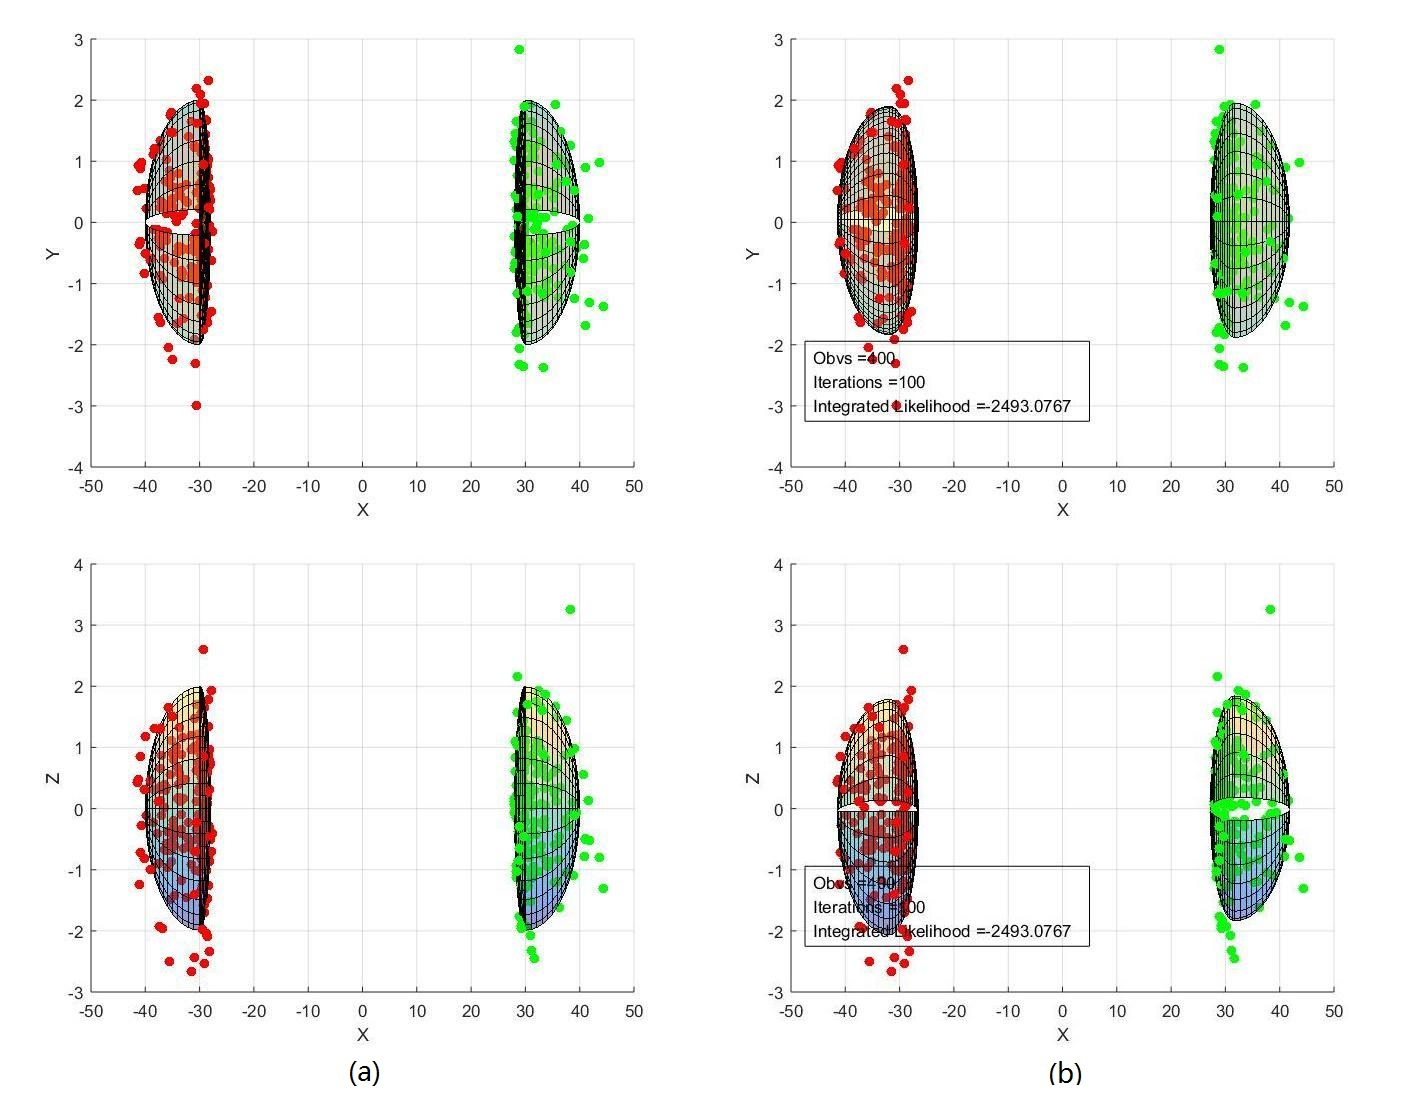
\includegraphics[width=0.4\paperwidth]{xyzMerge.jpg}
%\caption{(a) Original synthetic data grouping; (b) AGM clustering results}
%\label{fig:2}
%\end{figure}


%\begin{table*}[b]
%\caption{Original NSL-KDD data records}
%\begin{center}
%\begin{tabular}{|c|c|}
%\hline
%\multicolumn{1}{|p{1cm}|}{\centering\textbf{No}} & \multicolumn{1}{|p{10cm}|}{\centering\textbf{\textit{Value}}}\\
%\hline
%1 & {0,tcp,ftp\_data,SF,491,0,0,0,0,0,0,0,0,0,0,0,0,0,0,0,0,0,2,2,0.00,0.00,0.00,0.00,1.00,0.00,0.00,150,25,0.17,0.03,0.17,0.00,0.00,0.00,0.05,0.00,normal}\\
%2 & {0,udp,other,SF,146,0,0,0,0,0,0,0,0,0,0,0,0,0,0,0,0,0,13,1,0.00,0.00,0.00,0.00,0.08,0.15,0.00,255,1,0.00,0.60,0.88,0.00,0.00,0.00,0.00,0.00,normal} \\
%3 & {0,tcp,private,S0,0,0,0,0,0,0,0,0,0,0,0,0,0,0,0,0,0,0,123,6,1.00,1.00,0.00,0.00,0.05,0.07,0.00,255,26,0.10,0.05,0.00,0.00,1.00,1.00,0.00,0.00,neptune} \\
%4 & {0,tcp,http,SF,232,8153,0,0,0,0,0,1,0,0,0,0,0,0,0,0,0,0,5,5,0.20,0.20,0.00,0.00,1.00,0.00,0.00,30,255,1.00,0.00,0.03,0.04,0.03,0.01,0.00,0.01,normal} \\
%5 & {0,tcp,http,SF,199,420,0,0,0,0,0,1,0,0,0,0,0,0,0,0,0,0,30,32,0.00,0.00,0.00,0.00,1.00,0.00,0.09,255,255,1.00,0.00,0.00,0.00,0.00,0.00,0.00,0.00,normal} \\
%6 & {0,icmp,eco\_i,SF,18,0,0,0,0,0,0,0,0,0,0,0,0,0,0,0,0,0,1,1,0.00,0.00,0.00,0.00,1.00,0.00,0.00,1,16,1.00,0.00,1.00,1.00,0.00,0.00,0.00,0.00,ipsweep} \\
%\hline
%\end{tabular}
%\label{tab1}
%\end{center}
%\end{table*}
%
%\begin{table}[b]
%\caption{Accuracy Analysis ($M = 2$)}
%\begin{center}
%\begin{tabular}{|c|c|c|c|}
%\hline
%\multicolumn{1}{|p{1.5cm}|}{\centering \textbf{Component number $j = 1$}} & \multicolumn{1}{|p{1.5cm}|}{\centering \textbf{Mean \\($\mu_j$)}} & \multicolumn{1}{|p{1.5cm}|}{\centering \textbf{Left standard deviation ($\sigma_{lj}$)}} & \multicolumn{1}{|p{1.5cm}|}{\centering \textbf{Right standard deviation ($\sigma_{rj}$)}}\\
%\hline
%$\xi$ &-30.00, 0.00, 0.00&5.00, 1.00, 1.00&1.00, 1.00, 1.00\\
%$\hat{\xi}$ &-31.9, 0.05, -0.05&4.78, 0.94, 1.01&2.65, 0.92, 0.92\\
%\multicolumn{1}{|p{1.5cm}|}{\centering Euclidean Distance} & 1.882 & 0.226 & 1.657 \\
%\hline
%%\multicolumn{1}{|p{1.5cm}|}{\centering \textbf{Component number $j = 2$}} & \multicolumn{1}{|p{1.5cm}|}{\centering \textbf{Mean \\($\mu_j$)}} & \multicolumn{1}{|p{1.5cm}|}{\centering \textbf{Left standard deviation ($\sigma_{lj}$)}} & \multicolumn{1}{|p{1.5cm}|}{\centering \textbf{Right standard deviation ($\sigma_{rj}$)}}\\
%\hline
%$\xi$ &30.00, 0.00, 0.00&1.00, 1.00, 1.00&5.00, 1.00, 1.00\\
%$\hat{\xi}$ &31.70, 0.02, -0.01&2.24, 0.95, 0.91&5.06, 0.97, 0.93\\
%\multicolumn{1}{|p{1.5cm}|}{\centering Euclidean Distance} & 1.70 & 1.247 & 0.099 \\
%\hline
%\end{tabular}
%\label{tab2}
%\end{center}
%\end{table}



\noindent\textbf{Input:} Data observations $\mathcal{X}$ and component number $M$ \\
\textbf{Output:} AGM mixture parameter set $\Theta$
\begin{enumerate}
\item Initialization
\item Step $t$: For $t = 1,\ldots$
\begin{enumerate}
\item[]\textbf{Gibbs sampling part}
\item Generate $Z^{(t)}$ from Eq. \eqref{eq:memVector}
\item Compute $n_j^{(t)}$ from Eq. \eqref{eq:nj}
\item Generate $p_j^{(t)}$ from Eq. \eqref{eq:posterWeight}
\item[] \textbf{Metropolis-Hastings part}
\item Sample $\xi_j^{(t)}$ ($\mu_j^{(t)}, \sigma_{lj}^{(t)}, \sigma_{rj}^{(t)}$) from Eqs. \eqref{eq:posters}
\item Compute acceptance ratio $r$ from Eq. \eqref{eq:r}
\item Generate $\alpha = min[1,r]$ and $u \sim U_{[0,1]}$
\item If $\alpha \geq u$ then $\xi^{(t)} = \xi^{(t-1)}$
\item[] \textbf{RJMCMC part}
\item Generate $u' \sim U_{[0,1]}$. If $b_m>=u'$, perform split or birth step, then calculate acceptance probability $\mathcal{A}$. If the step is accepted, set $m=m+1$.
\item Generate $u' \sim U_{[0,1]}$. If $d_m>=u'$, perform merge or death step, then calculate acceptance probability $\mathcal{A}'$. If the step is accepted, set $m=m-1$.
\end{enumerate}
\end{enumerate}

\begin{figure}[b]
    \centering
    \begin{subfigure}[b]{0.22\paperwidth}
        \centering
        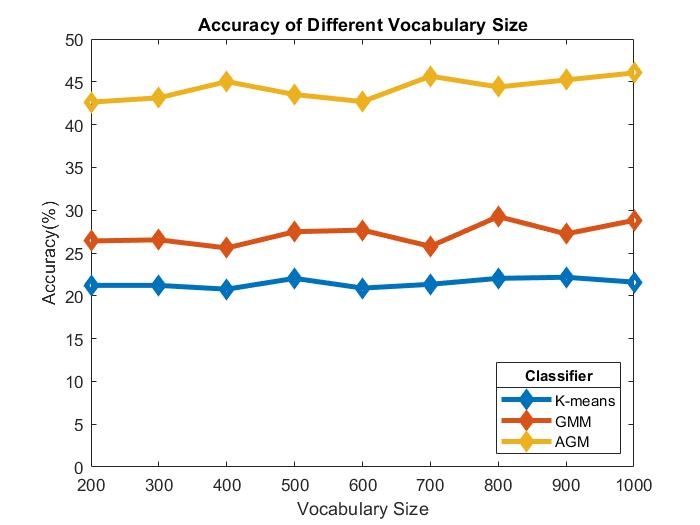
\includegraphics[width=0.20\paperwidth]{accurVoc.jpg}
        \caption{}
    \end{subfigure}
    \begin{subfigure}[b]{0.22\textwidth}
        \centering
        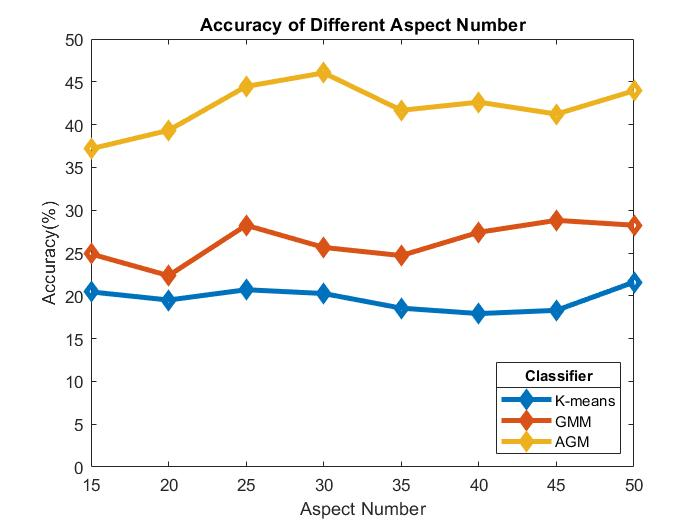
\includegraphics[width=0.20\paperwidth]{accurAspect.jpg}
        \caption{}
    \end{subfigure}
    \caption{a) Clustering accuracy by vocabulary size.  b) Clustering accuracy by latent aspect number.}\label{fig:3}
\end{figure}

\begin{figure}[b]
\centering
\includegraphics[width=0.42\paperwidth]{ConfMtx.jpg}
\caption{Confusion matrix of AGM model (Vocabulary size is 1000 and latent aspect number is 30)}
\label{fig:4}
\end{figure}
\section{Experimental results}
This section gives a detailed discussion around model adjustment, evaluation and effectiveness validation through the UIUC sports event dataset. A comparison is made between K-means, Gaussian mixture model (GMM) and proposed approach concerning different scenarios. Before apply the proposed model onto real dataset, hyperparameters related to the calculations of mixture weights and other parameters are set as follows: $\gamma_j = 1$ and both $\eta$ and $\tau$ are considered as $d$-dimensional zero vectors. Consequently, hyperparameters for priors of mixture parameters are set as follows\cite{Stephens2000}:
\begin{align}
\kappa = \frac{1}{\mathcal{R}^2}, \quad \alpha = 3, \quad g=0.3, \quad h=\frac{100g}{\alpha\mathcal{R}^2}
\label{eq:hypers}
\end{align}
where $\mathcal{R}$ is the interval of variation of observations.


%Theoretically, RJMCMC learning process should always be able to derive the optimal component number $M$. However, because of the stochastic sampling, improper proposal distributions or bad initialization parameters, learning result based on a single estimation run is not always satisfactory. In order to establish a robust parameter estimation algorithm, we evaluate the estimation outputs derived from multiple runs by calculating their marginal likelihood with the Laplace approximation\cite{Bouguila2009} on the logarithm scale which is defined as follows:
%
%\begin{multline}
%\log(p(\mathcal{X}|M)) = \log(p(\mathcal{X}|\hat{\Theta},M)) + \log(\pi(\hat{\Theta}|M)) \\
% + \frac{N_p}{2}\log(2\pi)+\frac{1}{2}\log(|H(\hat{\Theta})|)\qquad\quad
%\label{eq:margLikeli}
%\end{multline}
%where $\hat{\Theta}$ denotes the proposed optimal parameter set derived from a specific learning process and $\pi(\hat{\Theta}|M)$ is the prior density of mixture parameters as well as its Hessian matrix $H(\hat{\Theta})$ which is asymptotically equal to the posterior variance matrix.


%\begin{table}[b]
%\caption{Translation and Normalization of Internet Protocols (Enumerated Values)}
%\begin{center}
%\begin{tabular}{|c|c|c|}
%\hline
%\multicolumn{1}{|p{2cm}|}{\centering \textbf{Internet Protocols}} & \multicolumn{1}{|p{2cm}|}{\centering \textbf{\textit{Number of Occurrences}}} & \multicolumn{1}{|p{2cm}|}{\centering \textbf{\textit{Normalized Values}}}\\
%\hline
%ICMP & 1655 & 0\\
%UDP & 3011 & 0.071867 \\
%TCP & 20526 & 1 \\
%\hline
%\end{tabular}
%\label{tab3}
%\end{center}
%\end{table}
%
%\begin{table}[b]
%\caption{AGM Statistics}
%\begin{center}
%\begin{tabular}{|c|c|c|c|}
%\hline
%\multicolumn{1}{|p{1.5cm}|}{\centering \textbf{Init. Comp. Number}} & \multicolumn{1}{|p{1.5cm}|}{\centering \textbf{\textit{Estimated Comp. Number}}} & \multicolumn{1}{|p{1.5cm}|}{\centering \textbf{\textit{Accuracy}}} & \multicolumn{1}{|p{1.5cm}|}{\centering \textbf{\textit{Marginal Likelihood}}}\\
%\hline
%1 &2& 60.86\% & $-1.3596\mathrm{e}{6}$\\
%2 &2& 52.34\% & $-1.9886\mathrm{e}{6}$ \\
%3 &2& 53.39\% & $-2.2218\mathrm{e}{6}$ \\
%\hline
%\end{tabular}
%\label{tab4}
%\end{center}
%\end{table}
%
%\begin{table}[b]
%\caption{Confusion Matrices and Statistics of GMM and AGM}
%\begin{center}
%
%\begin{minipage}{0.75\textwidth}
%\begin{flushleft}
%\begin{tabular}{cc}
%
%\begin{minipage}{.3\textwidth} 
%\begin{center}
%\textbf{GMM} \\
%\begin{tabular}{|c|c|c|}
%\hline
% & \multicolumn{1}{|p{.7cm}|}{\centering \textbf{\textit{NF $^{\mathrm{a}}$}}} & \multicolumn{1}{|p{.7cm}|}{\centering \textbf{\textit{F $^{\mathrm{b}}$}}}\\
%\hline
%\multicolumn{1}{|p{.7cm}|}{\centering \textbf{\textit{NF}}} & 4238 & 7505\\
%\multicolumn{1}{|p{.7cm}|}{\centering \textbf{\textit{F}}} & 3397 & 10052\\
%\hline
%\end{tabular}
%\end{center}
%\end{minipage} &
%
%\begin{minipage}{.3\textwidth}    
%\begin{center}
%\textbf{AGM} \\
%\begin{tabular}{|c|c|c|}
%\hline
% & \multicolumn{1}{|p{.7cm}|}{\centering \textbf{\textit{NF}}} & \multicolumn{1}{|p{.7cm}|}{\centering \textbf{\textit{F}}}\\
%\hline
%\multicolumn{1}{|p{.7cm}|}{\centering \textbf{\textit{NF}}} & 2456 & 9278\\
%\multicolumn{1}{|p{.7cm}|}{\centering \textbf{\textit{F}}} & 582 & 12867\\
%\hline
%\end{tabular}
%\end{center}
%\end{minipage}  
%
%\end{tabular}
%\end{flushleft}
%\end{minipage}
%\end{center}
%
%\begin{center}
%\begin{tabular}{|c|c|c|}
%\hline
% & \multicolumn{1}{|p{1.5cm}|}{\centering \textbf{\textit{GMM}}} & \multicolumn{1}{|p{1.5cm}|}{\centering \textbf{\textit{AGM}}}\\
%\hline
%\multicolumn{1}{|p{2.5cm}|}{\centering \textbf{\textit{Accuracy}}}  & 53.39\% & 60.86\%\\
%\multicolumn{1}{|p{2.5cm}|}{\centering \textbf{\textit{Precision}}} & 36.09\% & 20.93\%\\
%\multicolumn{1}{|p{2.5cm}|}{\centering \textbf{\textit{False Positive Rate}}}  & 42.75\% & 41.90\%\\
%\multicolumn{1}{|p{2.5cm}|}{\centering \textbf{\textit{False Negative Rate}}} & 44.49\% & 19.16\%\\
%\hline
%\multicolumn{3}{l}{$^{\mathrm{a}}$Non fault-prone, $^{\mathrm{b}}$Fault-prone.}
%\end{tabular}
%\end{center}
%\label{tab5}
%\end{table}

\subsection{Image Categorization}
%
%\begin{figure}[b]
%\centering
%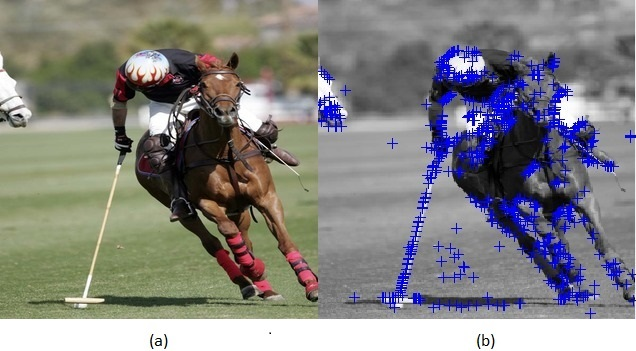
\includegraphics[width=0.4\paperwidth]{polo_merged.jpg}
%\caption{a) Original UIUC sport image b) Enhanced image with SIFT features}
%\label{fig:2}
%\end{figure}




A challenging UIUC sports event database\cite{Li2007} is selected for our target application which has been evaluated by previous researches \cite{Najar2018} \cite{Fan2011a}. It has 1579 images in total and consists of 8 sports event categories: rowing (250 images), badminton (200 images), polo (182 images), bocce (137 images), snowboarding (190 images), croquet (236 images), sailing (190 images), and rock climbing (194 images). The first step of image pre-processing is applying scale-invariant feature transform (SIFT) on the original image files using difference of Gaussian (DoG) \cite{Lowe1999} (Figure \ref{fig:2}) as interest point detector and then, visual feature will be translated into 128-dimensional feature descriptor vectors. Next, bag-of-visual-words (BOVW) \cite{Csurka2004} clusters feature vectors into a visual vocabulary $\mathcal{W}$ with variant vocabulary size using K-means algorithm. Consequently, each image will be represented by a frequency histogram of occurrence of visual words in $\mathcal{W}$. Since the vocabulary size in our test is between 200 to 1000, we also adopted probabilistic latent semantic analysis (pLSA) to describe each image as several latent topics (aspect) and therefore, reduce the dimension of image representation. Before applying AGM model for clustering, normalization based on feature scaling method is added to restrain the range of numerical attributes which will improve the Bayesian learning performance. Finally, we deploy the proposed AGM model as an unsupervised classifier to categorize the whole database. The proposed model is tested against image representation generated with different vocabulary size between 200 to 1000 with an interval of 100 and latent aspect number between 15 to 50 with an interval of 5 in order to identify the best accuracy.

According to a comparison between K-means, Gaussian mixture model (GMM) and proposed AGM model revels the fact that applying AGM to the sports event database leads to a significant clustering accuracy boost due to the best accuracy numbers of all the 3 classifiers illustrated in figure \ref{fig:3}(a) (K-means: 22.17\%, GMM: 29.26\% and AGM: 46.04\%). At the meanwhile, the impact of accuracy from different latent aspect numbers can be found in figure \ref{fig:3}(b).  Finally, the detailed clustering confusion matrix of AGM under the optimal vocabulary size (1000) and latent aspect number (30) is described in figure \ref{fig:4}.



%\begin{align}
%x' = \frac{x - min(x)}{max(x) - min(x)}
%\label{eq:normalize}
%\end{align}
%where $x$ and $x'$ are the attribute values before and after normalization as well as the maximum and minimum values $max(x)$  and $min(x)$. 


%We deploy our AGM model to the dataset with initial component number set between 1 and 3 and the learning iteration limit set to 30 loops. To better evaluate the performance and accuracy of our model under different initial number of components, at the end of each estimation, the fitting accuracy and marginal likelihood\cite{Bouguila2009} are recorded into Table \ref{tab4}. Obviously, the best result is the first run with initial component number equals to 1 which has the largest marginal likelihood value $-1.3596\mathrm{e}{6}$ and accuracy percentage 60.86\%. In order to better evaluate the model performance, the compared specifications derived from confusion matrices of AGM and GGM are shown in Table \ref{tab5}. In general, compared to GMM, AGM performs in a more accurate way for intrusion detection in terms of higher accuracy and much lower False Negative Rate indicating that AGM causes less false alarms of attack behaviors. However, it has a similar False Positive Rate and a lower precision value which means the intrusion detection abilities of both models are not satisfactory because of the absence of feature selection \cite{Bouguila2012b,Sheikhpour2017,Boutemedjet2007}. In addition, high-dimensional database will dramatically increase the noise during the clustering and eventually affect the usability of the model for real applications. Therefore, data-oriented model adjustment and dimensionality reduction techniques should be involved in order to mitigate this problem and achieve better detection outcomes.

\section{Conclusion and Future Work}
In this paper, we proposed a novel Bayesian framework based on asymmetric Gaussian mixture model via reversible jump Markov chain Monte Carlo method with feature selection and then, extended it to image categorization application which is a challenging UIUC sports event database. The proposed AGM model includes feature selection which can not only filters irrelevant and unneeded features but also weights relevant features based on the pertinent information they carry. For the parameter learning part, the proposed approach combines the merits of both Metropolis-Hastings and Gibbs sampling methods and allows model transfer throughout iterations by adopting RJMCMC methodology. A horizontal comparison between other unsupervised classifiers showing a significant accuracy improvement and future research directions will be focus on model adjustments and improvements to tackle high-dimensional datasets and achieve high clustering accuracy. 

%\section*{Appendix A}
%\subsection{Derivation of Acceptance Ratio $r$ by Eq. \eqref{eq:r}}
%The derivation of acceptance ratio $r$ is based on the assumption that mixture parameters are independent from each other which means that:
%\bigskip
%\begin{multline}
%\pi(\Theta) = \pi(p,\xi) = \pi(\xi) \\
%= \prod_{j=1}^M\pi(\mu_j)\pi(\sigma_{lj})\pi(\sigma_{rj}) \qquad\qquad\qquad\qquad\\
%= \prod_{j=1}^M\mathcal{N}_d(\mu_j|\eta,\Sigma)\mathcal{N}_d(\sigma_{lj}|\tau,\Sigma)\mathcal{N}_d(\sigma_{rj}|\tau,\Sigma)\quad
%\label{eq:14}
%\end{multline}
%in Eq. \eqref{eq:14}, since the mixture weigh $p$ is generated following Gibbs sampling method whose acceptance ratio is always 1, it should be excluded from Metropolis-Hastings estimation step. Accordingly, apply the same rule to the proposal distribution as well:
%\begin{multline}
%q(\Theta^{(t)}|\Theta^{(t-1)}) = q(\xi^{(t)}|\xi^{(t-1)})= \\
%\prod_{j=1}^M\mathcal{N}_d(\mu_j^{(t)}|\mu_j^{(t-1)},\Sigma)\mathcal{N}_d(\sigma_{lj}^{(t)}|\sigma_{lj}^{(t-1)},\Sigma)\mathcal{N}_d(\sigma_{rj}^{(t)}|\sigma_{rj}^{(t-1)},\Sigma)
%\label{eq:15}
%\end{multline}
%by combining Eqs. \eqref{eq:pdf} \eqref{eq:compPdf} \eqref{eq:posters} \eqref{eq:14} and \eqref{eq:15}, equation \eqref{eq:r} can be written as follows:
%
%\begin{multline}
%r = \frac{p(\mathcal{X}|\Theta^{(t)})\pi(\Theta^{(t)})q(\Theta^{(t-1)}|\Theta^{(t)})}{p(\mathcal{X}|\Theta^{(t-1)})\pi(\Theta^{(t-1)})q(\Theta^{(t)}|\Theta^{(t-1)})} \\
%= \prod_{i=i}^N \prod_{j=1}^M(\frac{p(X_i|\mu_j^{(t)},\sigma_{lj}^{(t)},\sigma_{rj}^{(t)})}
%{p(X_i|\mu_j^{(t-1)},\sigma_{lj}^{(t-1)},\sigma_{rj}^{(t-1)})} \qquad\qquad\qquad\\
%\times \frac{\mathcal{N}_d(\mu_j^{(t)}|\eta,\Sigma)\mathcal{N}_d(\sigma_{lj}^{(t)}|\tau,\Sigma)\mathcal{N}_d(\sigma_{rj}^{(t)}|\tau,\Sigma)}{\mathcal{N}_d(\mu_j^{(t-1)}|\eta,\Sigma)\mathcal{N}_d(\sigma_{lj}^{(t-1)}|\tau,\Sigma)\mathcal{N}_d(\sigma_{rj}^{(t-1)}|\tau,\Sigma)} \quad\\
%\times \frac{\mathcal{N}_d(\mu_j^{(t-1)}|\mu_j^{(t)},\Sigma)\mathcal{N}_d(\sigma_{lj}^{(t-1)}|\sigma_{lj}^{(t)},\Sigma)\mathcal{N}_d(\sigma_{rj}^{(t-1)}|\sigma_{rj}^{(t)},\Sigma)}{\mathcal{N}_d(\mu_j^{(t)}|\mu_j^{(t-1)},\Sigma)\mathcal{N}_d(\sigma_{lj}^{(t)}|\sigma_{lj}^{(t-1)},\Sigma)\mathcal{N}_d(\sigma_{rj}^{(t)}|\sigma_{rj}^{(t-1)},\Sigma)}
%\label{eq:16}
%\end{multline}

%\section*{Acknowledgment}
%The completion of this research work was made possible thanks to Concordia University via a Concordia University Research Chair Tier II.

\bibliographystyle{IEEEtran}
\bibliography{IEEEabrv,shuai}

\end{document}
